\documentclass[../full_thesis/full_thesis.tex]{subfiles}

% Default image directory
\newcommand{\thisdir}{../inertial_frame}
\graphicspath{{\thisdir/img/}}


\begin{document}

In Sec.~\ref{sec: rotating frame} we developed our intuition for the precession
of neutron stars by working in the rotating frame of the star. However, pulsar
astronomers report on direct observations of the radio pulsations in the
inertial frame. In this section, we will develop our precession model by making
predictions for how precession manifests in the observable features of a
pulsar. This will require us to understand and model the data collection
methods of pulsar astronomy. We will study each `physical observable'
separately and discuss how exact numerical results can be computed and derive
analytic approximations. \citet{Ruderman1970} first investigated phase modulation
due to precession, since then there has been extensive work in the literature:
\citet{Nelson1990} calculated phase residuals both analytically
and numerically for freely precessing stars; torqued precession was considered
for a general torque by \citet{Jones1988excitation} and \citet{Cordes1993} and
then for the \citet{Deutsch1955} torque by \citet{Melatos1999}. In this work,
we will closely follow the analytic results of \citet{Jones2001}. The novel
material here is in developing a numerical solution which allows direct
prediction of the physical observable features measured by observers, even
modelling the data collection mechanisms such as the observer-method to measure
$\dot{\nu}$. This chapter has two important aims: first, we want to develop our
intuition for precession which will be used in Chapter.~\ref{sec: testing
models}; second, this numerical model allows us to add physics into the model and
directly under the predictions it makes for observations. To demonstrate this,
we finish the chapter by showing some preliminary results of a model in which
the EM torque undergoes switching events as suggested by \citet{Lyne2010}.

\section{Introduction}
We begin by writing the moment of inertia as
\begin{align}
I^{a}_{\;\;b} = I_{0} \delta^{a}_{\;\;b} + \Delta I n^a n_b,
\end{align}
where $n^a$ is the \emph{deformation axis}, a unit vector pointing along the
body's symmetry axis. Then, if the body is biaxial about the $\z$ axis,
the angular momentum is given by
\begin{align}
J_{a} = I_0 \Omega_a + \Delta I \Omega_z n_a.
\end{align}
As discussed by \citet{Pines1972}, this shows that the three vectors $J_a$,
$\Omega_a$ and $n_a$ are always in the so-called reference plane as shown in
Fig.~\ref{fig: reference plane}.
\begin{figure}[htb]
    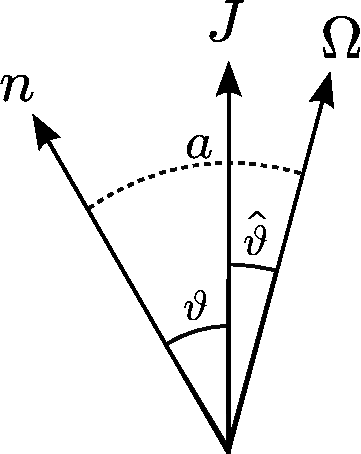
\includegraphics[width=0.2\textwidth]{ReferencePlane.pdf}
    \caption{The reference plane containing the angular momentum vector $\spin$,
    the angular momentum vector $\mathbf{J}$ and the symmetry axis $\mathbf{n}$ lying along the
    body-frame $\z$ axis. The dotted line indicates the polar angle $a$ between
    the body-frame $\z$ axis and the spin-vector.}
    \label{fig: reference plane}
\end{figure}
In this figure, we have defined the angle between anglular momentum and $n_a$ as
$\theta$, conventionally referred to as the \emph{wobble-angle} of
precession. We have also given $a$, the angle between the 3-axis and the
spin-vector as defined in Sec.~\ref{sec: rotating frame}.

From Eqn.~\eqref{eqn: rotation matrix} we can use these solutions to calculate
the motion of vectors fixed in the rotating frame, such as the magnetic
dipole, in the inertial frame. The results can display a rich
variety of behaviours which can be understood by decomposing the
spin-vector into rotation about the angular momentum and rotation about the
deformation axis:
\begin{equation}
  \spin = \dot{\phi}\n_{J} + \dot{\psi}\n_{d},
\label{eqn: decomp}
\end{equation}
where $\n_J$ and $\n_d$ are unit vectors along the angular momentum and deformation
axis as illustrated in Fig.~\ref{fig: reference plane}.
Any fixed vector in the rotating frame can be understood, in the inertial frame, as
undergoing two motions: keeping $\phi$ fixed and increasing $\psi$ rotates the
vector in a cone about the $\n_{d}$ axis; holding instead $\psi$ fixed and
increasing $\phi$ sweeps the vector about a cone centred around the $\n_{J}$
axis. Calling these cones the precession and spin cones respectively the
resulting motion can be understood as the superposition of the two.
\meta{CONNECT THESE TWO}
\citet{Jones2001} found that for nearly spherical stars where $\epsI \ll 1$
and when $\theta \ll 1$ the angles are related by
\begin{align}
\hat{\theta} \approx \epsI\theta.
\label{eqn: theta hat theta}
\end{align}
Consequently, from Fig.~\ref{fig: reference plane} we see that $a\approx
\theta$.

When including the EM torque, the wobble angle defined by \citet{Jones2001}
does not have the intuitive interpretation of the `amount' of precession.  In
particular, the anonalous part of the torque defined Eqn.~\eqref{eqn: torque}
can be understood to create an effective rotating frame as shown in Sec.~\ref{sec:
effective body frame}. This means that solutions exist which appear to undergo
`peristent precession' where $\theta \approx a\ne0$ such that the body remains
misaligned from the principal axes of its moment of inertia tensor. However, we
demonstrated that in fact the body has alligned with the principal axes of
it \emph{effective} moment of inertia tensor.

Let us then define a new wobble angle
\begin{align}
\wobbleangle = \theta - \beta.
\label{eqn: wobble angle}
\end{align}
That is, we rotate by the angle $\beta$ defined in Eqn.~\eqref{eqn: beta}. In
the limit where $\beta \rightarrow 0$ we recover the usual wobble angle referred
to by \citet{Jones2001} $\theta = \wobbleangle$, but if the effects of the
anomalous torque are important then our new wobble angle $\wobbleangle$ will
measure the amount of precession (i.e. its magnitude determines the amplitude
of precession).

\section{Rotating into the inertial frame}

The Euler rigid body equation of Eqn.~\eqref{eqn: eom} is defined in the
rotating frame of the star. To discuss results in the inertial frame of an
observer, we need to transform the solutions of Euler's rigid body equations
into the inertial frame.  An efficient way to do this is to determine the three
Euler angles which transform the rotating frame axes, denoted by $(x',y',
z')$, to the inertial frame axis, denoted by $(x, y, z)$. In particular, we
define three rotation matrices
\begin{align}
\begin{split}
D = \left[\begin{array}{ccc}
\cos\phi & \sin\phi & 0 \\
-\sin\phi & \cos\phi & 0 \\
0 & 0 & 1
\end{array}
\right],
\\
C = 
\left[\begin{array}{ccc}
1 & 0 & 0 \\
0 & \cos\theta & \sin\theta \\
0 & -\sin\theta & \cos\theta
\end{array}
\right], \\
B = \left[\begin{array}{ccc}
\cos\psi & \sin\psi & 0 \\
-\sin\psi & \cos\psi & 0 \\
0 & 0 & 1
\end{array}
\right].
\end{split}
\end{align}
Then their product defines the Euler angle rotation matrix
\begin{align}
\begin{split}
R(\theta, \phi, \psi) & = BCD \\
& \left[
\begin{array}{ccc}
\cos\psi \cos\phi - \cos\theta \sin\phi \sin \psi &
\cos\psi \sin \phi + \cos\theta \cos \psi \sin \psi &
\sin \psi \sin\theta \\
-\sin\psi \cos\phi - \cos\theta\sin\phi\cos\psi &
-\sin\psi\sin\phi + \cos\theta\cos\phi\cos\psi &
\cos\psi \sin\theta \\
\sin\theta\sin\phi &
-\sin\theta \cos\phi &
\cos\theta
\end{array}
\right].
\end{split}
\label{eqn: rotation matrix}
\end{align}
Here we are using the
$(\phi, \theta, \psi)$ Euler
angle parameterisation as described by \citet{Landau1969}; a diagram of how
these angles is given in Fig.~\ref{fig: Euler}.\begin{figure}[ht]
\centering
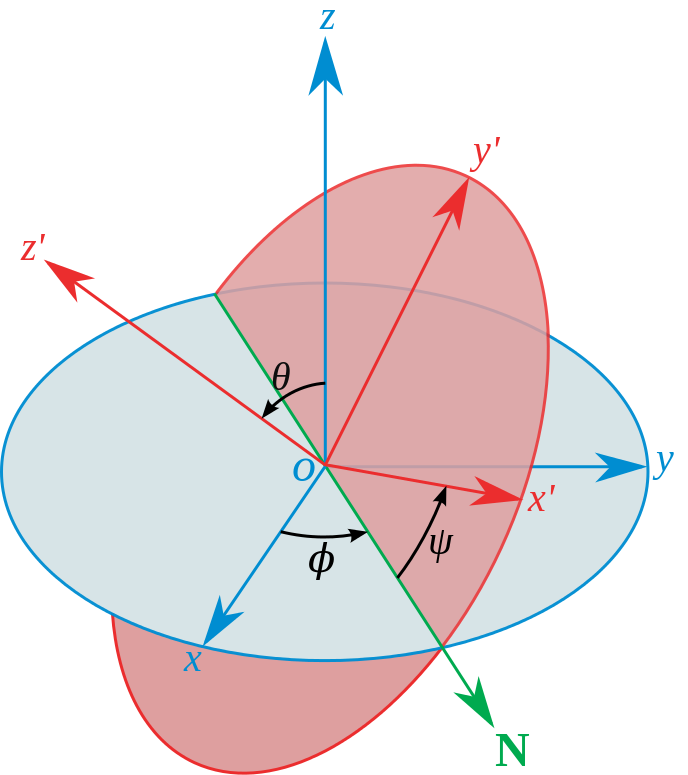
\includegraphics[scale=0.25]{Eulerangles-alternative_filled.png}
\caption{Schematic of the Euler rotation angles between the rotating 
frame $(x', y', 'z')$ and the inertial frame $(x, y, z)$. Image courtesy of
 \citet{WikipediaEuler}.}
\label{fig: Euler}
\end{figure}
This matrix, given values for the Euler angles, transforms from the fixed
interial system of coordinates to the rotating frame. So for $A^{\textrm{in}}$,
a vector defined in the inertial frame, in the rotating frame this has
components given by
\begin{align}
A^{\textrm{rot}}_{a} = R^{b}_{\;\;a} A^{\textrm{in}}_{b}.
\end{align}


The Euler angles themselves will evolve with time. To calculate this, we express
the components of $\Omega$ along the moving axes ($x', y', z')$. As shown by
\citet{Landau1969} this results in a set of three ODEs which are coupled both to
the other Euler angles and the components of the spin-vector. To have solutions
both for the motion of the spin-vector in the rotating frame and the Euler
angles we need to solve all six ODEs together. To be specific, the six ODEs are
given in equations~\eqref{eqn: ODEs}: in the left-hand triplet is the
components of the Euler rigid body equations first given in Eqn.~\eqref{eqn:
eom}; in the right-hand triplet we give the rearranged set of Euler angles ODEs
from \citet{Landau1969}.
\begin{align}
\begin{split}
\dot{\omega}_{x} & = \frac{1}{I_{xx}}\left[T_{x} +
                      \left(I_{yy} - I_{zz}\right) \omega_{y} \omega_{z}\right],
\\
\dot{\omega}_{y} & = \frac{1}{I_{yy}}\left[T_{y} +
                      \left(I_{zz} - I_{xx}\right) \omega_{x} \omega_{z}\right],
\\
\dot{\omega}_{z} & =\frac{1}{I_{zz}}\left[T_{z} +
                      \left(I_{xx} - I_{yy}\right) \omega_{x} \omega_{y}\right],
\end{split}
\begin{split}
\dot{\phi} & = \frac{\omega_{x} \sin \psi + \omega_{y} \cos \psi}{\sin \theta},\\
\dot{\theta} & = \omega_{x} \cos \psi - \omega_{y} \sin \psi,\\
\dot{\psi} & = \omega_{z} - \dot{\phi} \cos \theta.
\end{split}
\label{eqn: ODEs}
\end{align}
This set of six coupled ODEs can be solved numerically using a time stepper; we
will use the \texttt{rkf45} stepper provided by GSL \citep{gough2009gnu}.
Solutions give the components of the spin-vector in the rotating frame and the
evolution of the Euler angles which can be used to transform rotating frame
quantities into the inertial frame. Unlike the results of Sec.~\ref{sec:
rotating frame}, numerical solutions to these ODEs require the fast spin frequency
to be resolved and hence require greater computing time.

%The rotation period of the star is several orders of magnitude smaller than the
%precession period, as a result the Euler angles evolve on a much shorter time
%scale than the rotating frame spin components. This is numerically expensive. To
%allow efficient investigations we will therefore consider unrealistic values to
%understand the different types of motion before using realistic values only in
%cases of interest.

\section{Initial conditions}
\label{sec: initial conditions}

Solving the rigid body equations, as in Sec.~\ref{sec:
rotating frame}, we impose the following initial conditions on the
spin vector
\begin{align}
\omega_{x} & = \omega_{0}\sin(a_{0}), &
\omega_{y} & = 0, &
\omega_{z} & = \omega_{0}\cos(a_{0}),
\label{eqn: spin init}
\end{align}
such that $\spin(t=0)$ lies in the $x' - z'$ plane at an angle $a_{0}$ to the
$z'$ axis.

For the Euler angle equations, the right-hand triplet in Eqn.~\eqref{eqn:
ODEs}, the initial conditions need to be chosen carefully so that the result
can be meaningfully interpreted. In particular, we need to be sure we understand
how the inertial frame is orientated. Let us note that the angular
momentum in the two frames are related by
\begin{equation}
\Jr_a = R^{b}_{\;\;a} \Ji_b .
\label{eqn: transform}
\end{equation}
where $R^{a}_{\;\;b}$ is defined in Eqn.~\eqref{eqn: rotation matrix}.

In the rotating frame, the moment of inertia is constant except for small variations
due to the fact that the torque is not parallel to the angular momentum.
We have already set the initial condition on $\spin$ in Eqn.~\eqref{eqn:
spin init}, therefore the initial angular momentum in the rotating frame is given by
\begin{equation}
  \Jr_a(t=0) = I \omega_a(t=0).
\end{equation}
If we set an initial condition on the angular momentum in the inertial frame
$\Ji$ then Eqn.~\eqref{eqn: rotation matrix} uniquely defines the initial
Euler angles. We choose to set the initial angular momentum in the inertial
frame to lie along the inertial $z$ axis such that
\begin{equation}
  \Ji_a(t=0) = |\Ji| \hat{z}.
\end{equation}
The magnitude of the angular momentum is
\begin{equation}
|J| = |I \omega_{a}|=\omega_{0}\sqrt{(I_{xx}\sin a_{0})^{2} + (I_{zz}\cos a_{0})^{2}},
\end{equation}
then substituting into Eqn.~\eqref{eqn: transform} we have
\begin{equation}
\left[ \begin{array}{c}
I_{xx}\sin a_{0} \\
0 \\
I_{zz} \cos a_{0}
\end{array}\right] =
\sqrt{(I_{xx}\sin a_{0})^{2} + (I_{zz}\cos a_{0})^{2}}
\left[ \begin{array}{c}
\sin \psi_{0} \sin \theta_{0} \\
\cos \psi_{0} \sin \theta_{0} \\
\cos \theta_{0}
\end{array}\right].
\label{eqn: 010203}
\end{equation}
This gives us three equations for two unknowns. Our choice to set $\Ji$ along
the $z$ axis leaves the initial value of $\phi$ a free variable,
we set $\phi(t=0) = 0$ without loss of generality.
Rearranging the third component of Eqn.~\eqref{eqn: 010203} yields
\begin{equation}
\theta_{0} = \arccos\left(\frac{I_{zz}\cos a_{0}}{ \sqrt{(I_{xx}\sin
        a_{0})^{2} + (I_{zz}\cos a_{0})^{2}}} \right).
\label{eqn: theta init}
\end{equation}
In the limit $\epsilon_{I} \ll 1$ we have that $\theta_{0} \approx a_{0}$.
For $\psi_0$, we rearrange the first component of Eqn.~\eqref{eqn: 010203} to
give
\begin{equation}
\sin\psi_{0} =\frac{1}{ \sin\theta_{0}}
\frac{ I_{xx}\sin a_{0}}{\sqrt{(I_{xx}\sin a_{0})^{2} + (I_{zz}\cos a_{0})^{2}}}.
\label{eqn: 8283}
\end{equation}
To simplify the first factor we use the identity $\sin(\arccos(x)) = \sqrt{1 - x^{2}}$
along with Eqn.~\eqref{eqn:  theta init} giving
\begin{equation}
\sin\theta_{0} = \left(\frac{(I_{xx}\sin a_{0})^{2}}
                  {(I_{xx}\sin a_{0})^{2} + (I_{zz}\cos a_{0})^{2}} \right)^{1/2}.
\end{equation}
Inserting this into Eqn.~\eqref{eqn: 8283} and rearranging we find that
\begin{align}
\sin \psi_0 & = \frac{I_{xx} \sin a_{0}}{\left(I_{xx}^{2} \sin^{2} a_{0}\right)^{1/2}} \\
 & = \frac{\sin a_{0} }{|\sin a_{0}|} \\
& = \mathrm{sign}(a_{0}),
\end{align}
where by $\mathrm{sign}(x)$ we mean the sign of $x$. Finally, the initial
condition is given by
\begin{align}
\psi_{0} & =\mathrm{sign}(a_{0}) \frac{\pi}{2}.
\label{eqn: psi  init}
\end{align}
We can check the sanity of this result by inserting it into the second component of
Eqn.~\eqref{eqn: 010203} and finding that it balances the left hand side.

In this section, we have defined the appropriate initial conditions for the
system: in addition to Eqn.~\eqref{eqn: spin init} defining the initial spin-vector,
we set the angular momentum in the inertial frame to lie along the
$z$ axis and fix $\phi(t=0)=0$ without loss of generality.  While the
initial conditions on the spin-vector are arbitrary, if the initial Euler angle
are not carefully defined then we do not have a meaningful interpretation for
how the inertial frame is orientated.

\section{Dynamics of the magnetic dipole}

Numerical solutions to Eqn.~\eqref{eqn: ODEs} allow us to calculate the motion
of any quantity in the inertial frame from which the neutron star is observed.
This can be used for example to calculate the motion of the spin-vector in the
rotating frame under any torque. However, pulsar astronomers observe the pulsar
through the pulsations of EM emission. If this emission is colinear with the
dipole, then it points along the unit vector of the magnetic dipole $\m$. Therefore,
we are particular interested in the motion of $\m$ in the inertial frame.

In the rotating frame, we set $\m$ to lie at an angle $\chi$ to the $z'$ axis
with unit vector $[\sin(\chi), 0, \cos(\chi)]$ without loss of generality.
Using the inverse of Eqn.~\eqref{eqn: rotation matrix}, the Euler angles rotation matrix, we
can transform to the inertial frame; the components of the magnetic dipole in
the inertial frame are
\begin{equation}
\m =
\left[\begin{array}{c}
\cos\phi\cos\psi\sin\chi - \sin\phi \cos \theta \sin \psi \sin \chi
+ \sin \phi \sin \theta \cos \chi \\
\sin\phi\cos\psi\sin\chi + \cos\phi \cos \theta \sin \psi \sin \chi
- \cos \phi \sin \theta \cos \chi \\
\sin\theta \cos\psi \sin\chi + \cos\theta \cos \chi
\end{array}\right].
\label{eqn: m inertial}
\end{equation}•
Following the work of \citet{Jones2001} we define two angles $\Phi$ and $\Theta$
which describe the polar and azimuth of $\m$ in the inertial frame.
From Eqn.~\eqref{eqn: m inertial} the azimuthal angle is given by
\begin{equation}
    \Phi = \arctan\left(\frac{\m_{y}}{\m_{x}}\right) =
\phi - \frac{\pi}{2} + \arctan\left(\frac{1}{\cos\theta}
                       \left(\frac{\cos\psi \tan \chi}{\tan\theta -
                       \sin \psi \tan\chi }\right)\right),
\label{eqn: Phi}
\end{equation}
while the polar angle is
\begin{equation}
\Theta = \arccos(\m_{z}) = \arccos(\sin \theta \sin \psi \sin \chi + \cos \theta \cos \chi ).
\label{eqn: Theta 2}
\end{equation}

Given a numerical solution of equations~\eqref{eqn: ODEs}, i.e. the evolution
of the spin-vector and three Euler angles, we can use these two equations to
describe the evolution of the magnetic dipole orientation in the inertial
frame. Before doing so, we will consider what can be learnt analytically in the
torque free case.

\subsection{Torque free precession}

Using our numerical solution, we simulate a star without any EM torque. The
resulting solutions for the Euler angles can then be substitued into Eqn.~\eqref{eqn: Theta 2}
to give the evolution of $\Theta$. This is done for three choices of $\theta$
and $\chi$ in Fig.~\ref{fig: polar angle variations}. The significance of these
choices will be discussed in the next section.
\begin{figure}[ht]
\centering
  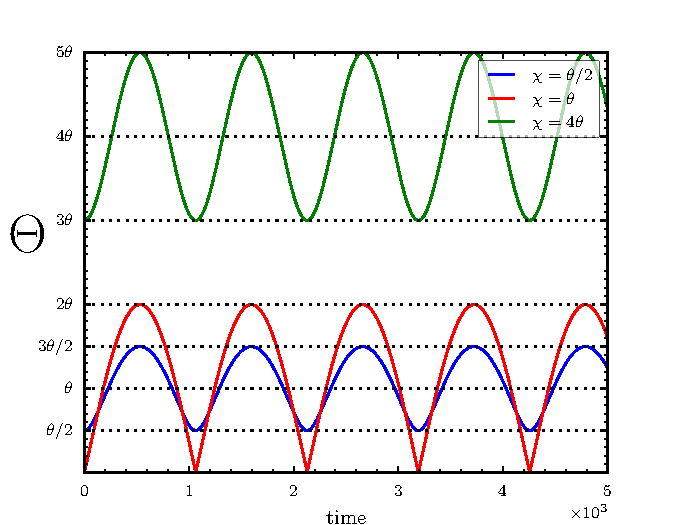
\includegraphics[width=0.7\textwidth]{polar_angle_variation_with_chi.pdf}
\caption{Variations in the polar angle of the dipole $\m$ under free precession}
\label{fig: polar angle variations}
\end{figure}

The spin frequency of a pulsar is the rate with which observers measure the
observed pulsations, usually we think of this as exactly the rotation frequency
$\omega$. However, for a precessing star the observed frequency is not given by
$\omega$ due to the additional motions of precession. Instead, we note that the
observer would fit a timing model to the TOAs as the pulse passes through the
plane containing them and the angular momentum vector, the phase of which is
$\Phi$. So the frequency measured would be given by the first derivative of $\Phi$:
\begin{equation}
\dot{\Phi} = \dot{\phi}
+ \frac{\sin\chi \left(
\dot{\psi} (\cos\theta\sin\chi - \sin \psi \sin \theta \cos\chi) +
\dot{\theta} \cos\psi (\cos\theta\cos\chi - \sin \psi \sin \theta \sin\chi)\right)
}{(\sin\theta \cos \chi - \cos \theta \sin \psi \sin \chi)^{2} + \cos^{2}\psi \sin^{2} \chi}.
\label{eqn: Phi_dot}
\end{equation}
This is the \emph{instantaneous electromagnetic frequency}; an observer
will measure the time averaged value of $\dot{\Phi}$ as the `spin frequency' of
the star.

In Fig.~\ref{fig: frequency variations} we plot the frequency modulations for the
three free precession cases discussed in Sec.~\ref{sec: understanding the motion of m}.
\begin{figure}[ht]
\centering
  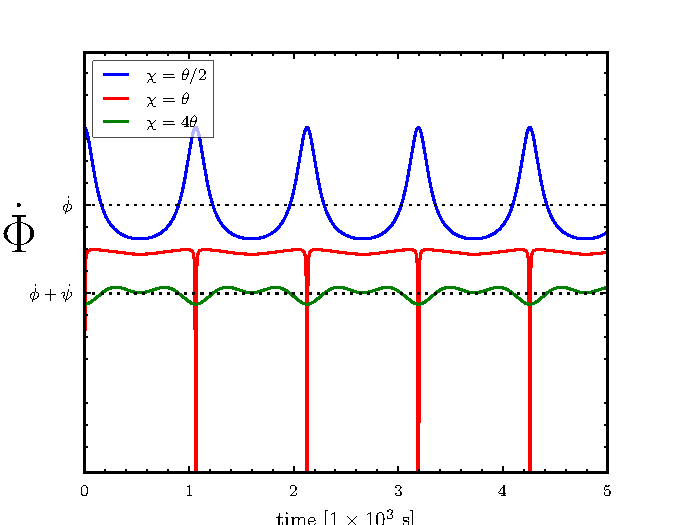
\includegraphics[width=0.7\textwidth]{frequency_variation_with_chi.pdf}
\caption{Variations in the instantaneous electromagnetic frequency for three choices
of $\chi$ and $\theta$ under free precession}
\label{fig: frequency variations}
\end{figure}
Additionally for the two cases $\chi>\theta$ and $\chi < \theta$ we have
plotted the average spin frequencies $\dot{\phi}$ and $\dot{\phi}+\dot{\psi}$
as predicted by \citet{Jones2001}. This shows the periodic modulations in all
three instances, and the instantaneous drop in spin frequency to zero in the
case of $\chi=\theta$.



The solutions to equations~\eqref{eqn: ODEs} were studied by \citet{Jones2001}
where it was found that the Euler angles had simple analytic solutions given by
\begin{align}
\begin{split}
    \theta(t) & = \theta_{0} \approx a_{0}, \\
    \phi(t) & = \dot{\phi}t + \phi_{0} = \dot{\phi} t, \\
    \psi(t) & = \dot{\psi}t + \psi_{0}=
 -\frac{\Delta I}{I_0}\dot{\phi} t + \textrm{sign}(a_0)\frac{\pi}{2},
\end{split}
\label{eqn: euler angles torque free evolution}
\end{align}
where in the second step we have inserted the initial conditions.  Solutions to
the rigid body equations in the absense of a torque can be found in
Eqn.~\eqref{eqn: free precession}.



\subsection{Understanding the motion of $\m$}
\label{sec: understanding the motion of m}
\citet{Jones2001} found that the types of solutions these cones produced
depended on whether $\theta < \chi$ or $\theta > \chi$. To understand why this is, in
Fig.~\ref{fig: cones} we provide three illustrations of the two cones projected
into the reference plane (see Fig.~\ref{fig: reference plane}) for the three
possible orderings of $\theta$ and $\chi$ ($\chi < \theta$, $\chi=\theta$, $\chi > \theta$).
\begin{figure}[ht]
\centering
	\subfloat[$\chi < \theta$]{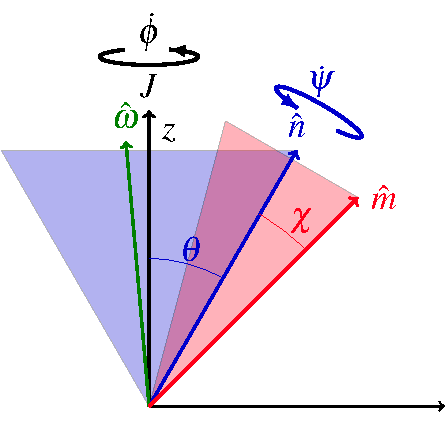
\includegraphics[width=0.33\textwidth]
    {chi_less_theta.pdf}}
	\subfloat[$\chi = \theta$]{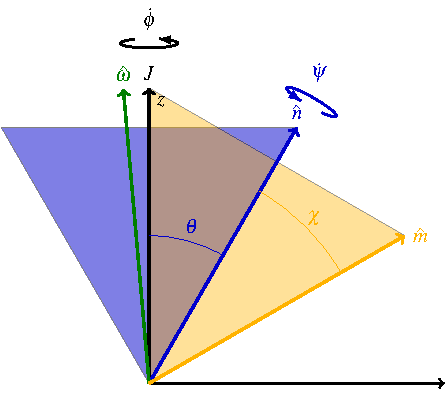
\includegraphics[width=0.33\textwidth]
    {chi_equal_theta.pdf}}
	\subfloat[$\chi > \theta$]{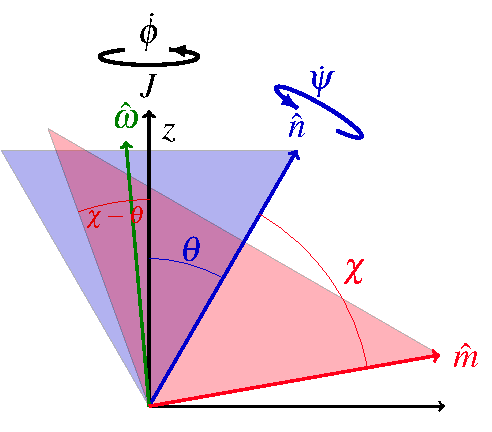
\includegraphics[width=0.33\textwidth]
    {chi_more_theta.pdf}}
\caption{Diagrams depicting 2D projections of the cones swept out by the
    different motions under torque free precession onto the reference plane.
    The yellow cone is swept out by the rotation of $\m$ about $\n_{d}$ at the
    slow precession frequency; the blue cone is swept out by the rotation of
    $\n_{d}$ about $\J$ at the fast spin frequency. For oblate bodies the
precession cone rotates in the opposing direction to the spin cone.}
\label{fig: cones}
\end{figure}

The motion of the magnetic dipole about the precession cone evolves on a much
longer timescale than its motion about the spin cone; as a result the star will
always pulsate once every spin period, but the long precession will modulate
the average value on the precession timescale. Because of the large difference
in timescales, the motion of $\m$ can be considered as the slow evolution of a
third cone swept out by $\m$ about $\J$ which we will call the \emph{dipole cone}. The
half angle made by this cone is exactly the polar angle $\Theta$ which we derive
later in Eqn.~\eqref{eqn: Theta 2}. The frequency with which $\m$ rotates around
dipole cone is $\dot{\Phi}$ given by Eqn.~\eqref{eqn: Phi_dot}. Let us now
describe the evolution of the dipole cone for the three cases in Fig.~\ref{fig: cones}:
\begin{itemize}
\item The $\chi < \theta$ case ($\chi = \theta/2$): the precession cone is narrow and does not
extend over the angular momentum vector. The polar angle $\Theta$ of the dipole
cone oscillates periodically between $\theta+\chi$ and $\theta-\chi$
during a precession cycle. The spin frequency $\dot{\Phi}$ has an average value
of $\dot{\phi}$ and
oscillates about this value, comparing with the $\Theta$ variations
demonstrates these oscillations are locked in phase with the rotation of $\m$
in the precession cone. Recalling that the precession cone counter rotates with
respect to the spin cone, at $\theta+\chi$ the precession cone motion acts in
the opposing direction to the spin cone, this causes a reduction in the spin
frequency away from the average; by contrast at $\theta+\chi$ the counter
rotation is now in favour of the spin frequency and as a result the spin
frequency is increased above the average.

\item The $\chi = \theta$ case: in this special case the angular momentum vector sits exactly
on the side of the precession cone, this suggest at certain precessional phases $\m$ can align exactly with
the angular momentum. When this happens the spin frequency tends to zero manifesting as sharp dips in the
spin frequency; at the same time the polar angle tends to zero.

\item The $\chi > \theta$ case ($\chi = 4\theta$): The precession cone now extends over the
angular momentum vector, this means it always acts to reduce the spin
frequency; as a result the spin frequency has an average value of
$\dot{\phi} + \dot{\psi}$. The polar angle can vary between $\theta+\chi$ and
$\chi-\theta$, for $\chi$ close to $\theta$ the deviations away from the
average are large while as $\chi$ increases the deviations get smaller as
the half angle of the dipole cone increases.
\end{itemize}
We will comment on these results further by verifying them numerically in
Fig.~\ref{fig: polar angle variations} and Fig.~\ref{fig: frequency variations}.

Finally, we need to relate the decomposed angular
velocities $\dot{\phi}$ and $\dot{\psi}$ to the physical properties of the
model.  This can be done from Eqn.~\eqref{eqn: decomp} by recalling that
$\theta$ is the angle between the angular momentum and the deformation axis
(see Fig.~\ref{fig: reference plane}) and then applying the cosine rule
\begin{align}
|\spin|^{2} = \dot{\phi}^{2}+\dot{\psi}^{2} - 2\dot{\phi}\dot{\psi}\cos\theta.
\end{align}
From \citet{Jones2001}, when $\epsI \ll 1$ the two are related by
\begin{align}
\dot{\psi} \approx - \epsI \dot{\phi},
\label{eqn: psi dot}
\end{align}
and so rearranging we find that
\begin{align}
\dot{\phi} = \frac{|\spin|}{\sqrt{1+\epsI^{2} - 2\epsI\cos\theta}}.
\label{eqn: phi dot}
\end{align}

\section{Evolution of the Euler angles for a torque free biaxial body}
\label{sec: biaxial body with no torque}

In Eqn.~\eqref{eqn: euler angles torque free evolution} we saw that
\citet{Jones2001} had derived analytic solutions for the Euler angle evolution
in which the wobble angle $\theta$ remains fixed; the azimuthal angle $\phi$
monotonically increases at $\dot{\phi}$ which from Eqn.~\eqref{eqn: phi dot} is
approximately the spin frequency; while the rotating frame precession refers to the
linear change in $\psi$ at the precession frequency $\dot{\psi}$ related to the
spin frequency by Eqn.~\eqref{eqn: psi dot}. This set of analytic solutions gives
us a method to verify our numerical solver of Eqn.~\eqref{eqn: ODEs} with the
appropriate initial conditions.

In Fig.~\ref{fig: biaxial body no torque} we present the Euler angle solutions
of equation \eqref{eqn: ODEs} for some arbitrary values.  This demonstrates
`almost' perfect agreement with \citet{Jones2001} for the Euler angles of a
oblate precessing body. That is, $\phi$ monotonically increases at the spin
frequency while $\psi$ decreases at the slower precession frequency. The polar
angle $\theta$ should remain constant during this simulation. Inspecting its
value however, we find it varies fractionally by $\sim 10^{-11}$.  This is
caused by the finite numerical precision when performing the subtraction in
equation \eqref{eqn: ODEs} for $\dot{\theta}$. On short time scales, these
errors remain small; over sufficiently long time scale these errors can
accumulate and eventually lead to a complete loss of numerical accuracy. We
must therefore be vigilant to ensure this does not occur when considering
realistic values.
\begin{figure}[htb]
    \centering
\subfloat[Spherical components in the rotating frame]
         {\includegraphics[width=0.7\textwidth]
         {{Spherical_Plot_Unknown_SpindownTorqueSwitching_1_chi0_8.0000000000e+01_omega0_1.00e+01_epsI3_1.00e-03_AnomTorqueSwitching_1_n_10000_a0_1.5000000000e+01_T_5.00e+03_upsilon_0.00e+00_epsA_0.00e+00_epsI1_0.00e+00_AnomTorque_1}.pdf}} \\
\subfloat[Euler angles ]
         {\includegraphics[width=0.7\textwidth]
         {{Euler_Angles_Unknown_SpindownTorqueSwitching_1_chi0_8.0000000000e+01_omega0_1.00e+01_epsI3_1.00e-03_AnomTorqueSwitching_1_n_10000_a0_1.5000000000e+01_T_5.00e+03_upsilon_0.00e+00_epsA_0.00e+00_epsI1_0.00e+00_AnomTorque_1}.pdf}}
\caption{Solution to the ODEs defined in Eqn.~\eqref{eqn: ODEs} for a
torque free biaxial NS with a deformation of $\epsI = 10^{-3}$. The red
dashed line is the analytic calculation found by \citet{Jones2001} for the
evolution of the Euler angles as given in Eqn.~\eqref{eqn: euler angles torque free evolution}.}
\label{fig: biaxial body no torque}
\end{figure}

\section{Evolution of the Euler angles for a torqued biaxial body}
To see the difference introducing the EM torque of Eqn.~\eqref{eqn: torque}  makes to the
solutions, in Fig.~\ref{fig: biaxial body with torque} we repeat the simulation
plotted in Fig.~\ref{fig: biaxial body no torque} with both the anomalous
and spin-down components of the EM torque. The most
striking contrast is the `wobble' in both $\theta$ and $a$, on closer
inspection one also finds this wobble in the other angles, while the magnitude of
$\spin$ both wobbles and undergoes a secular spin down.
\begin{figure}[ht]
    \centering
\subfloat[Spherical components in the rotating frame]
         {\includegraphics[width=0.7\textwidth]
         {{Spherical_Plot_Unknown_SpindownTorqueSwitching_1_chi0_8.0000000000e+01_omega0_1.00e+01_epsI3_1.00e-03_AnomTorqueSwitching_1_n_10000_a0_1.5000000000e+01_T_5.00e+03_upsilon_0.00e+00_epsA_5.00e-04_epsI1_0.00e+00_AnomTorque_1}.pdf}} \\
\subfloat[Euler angles]
         {\includegraphics[width=0.7\textwidth]
{{Euler_Angles_Unknown_SpindownTorqueSwitching_1_chi0_8.0000000000e+01_omega0_1.00e+01_epsI3_1.00e-03_AnomTorqueSwitching_1_n_10000_a0_1.5000000000e+01_T_5.00e+03_upsilon_0.00e+00_epsA_5.00e-04_epsI1_0.00e+00_AnomTorque_1}.pdf}}
\caption{Solution to the ODEs defined in Eqn.~\eqref{eqn: ODEs} including the
torque defined in Eqn.~\eqref{eqn: torque} for a biaxial body with
$\epsA=\epsI/2$ and $\epsI=1\times10^{-3}$. Note the x-axis is in units of
$\tauP$, the initial precession period.}
\label{fig: biaxial body with torque}
\end{figure}

These solutions show that our numerical simulation is capable of solving the
set of coupled ODEs presented in Eqn.~\eqref{eqn: ODEs} including the effects
of the torque. In the following sections we will discuss methods to calculate
the `physical observables' which pulsar astronomers report on.

%\paragraph{Convergence test}
%To ensure that the small wobble in $\theta$, which should remain constant, is
%a numerical effect rather than a lack of physics we can plot the fractional
%size of the wobble whilst changing the absolute error tolerance given to the
%ODE stepping procedure. This is done in figure \ref{fig: error}
% \begin{figure}[ht]
%\centering
%\includegraphics[scale=0.4]{error_plot.pdf}
%\caption{Fractional size of variations in theta plotted against the relative
%error tolerance given to the stepper.}
%\label{fig: error}
%\end{figure}
%We observe a strange behaviour in which the magnitude of the fractional difference, defined by
%\begin{equation}
%\textrm{Var}(\theta) = \frac{\theta_{\textrm{max}} - \theta_{\textrm{min}}}{|\theta|},
%\end{equation}
%increases exponentially as the error becomes very small. This is due to a
%change in the type of variation of theta, for larger absolute errors we
%observe a period wobble around the expected value of $\theta$. In contrast for
%much smaller absolute errors the solution seems to wander of the mean value
%whilst also undergoing a periodic wobble. We demonstrate this in figure
%\ref{fig: error example} for the two extremes values.
%
%\begin{figure}[ht]
%\centering
%\includegraphics[scale=0.4]{error_example.pdf}
%\caption{Resulsts of simulations with different error tolerances,
%interestingly the smaller absolute error produces greater numerical
%inaccuracy.}
%\label{fig: error example}
%\end{figure}


%\subsection{Pulse frequency and polar angle under torqued precession}
%Having a physical understanding of why $\Theta$ and $\dot{\Phi}$ evolve under
%free precession as in Fig.~\ref{fig: polar angle variations} and Fig.~\ref{fig:
%frequency variations}, we will study what happens to such a system when
%including the effects of the EM torque.
%
%In Fig.~\ref{fig: polar angle variations with torque}  we give the variations in
%the polar angle under torqued precession.The torque introduces two
%additional effects: $\dot{\Phi}$ the instantaneous electromagnetic frequency
%decays slowly, this is caused by the spin down torque and is full agreement
%with what we expect; a fast sinusoidal oscillation in $\dot{\Phi}$ on the spin
%time scale, observable as a broadening of the line, is a result of the
%anomalous torque. As for the polar angle $\Theta$ the anomalous torque causes
%slight changes in the limits of the sinusoidal variation. Both the anomalous
%torque effects can be understood by realising that this effectively adds a
%triaxiality into the moment of inertia tensor. % needs more explanation
%
%\begin{figure}[ht]
%\centering
%	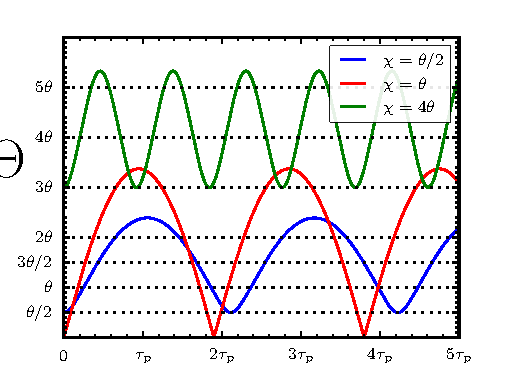
\includegraphics[width=0.7\textwidth]{polar_angle_variation_with_chi_inc_torque.pdf}
%\caption{Variations in the polar angle of the dipole $\m$ under torqued precession}
%\label{fig: polar angle variations with torque}
%\end{figure}
%
%\begin{figure}[ht]
%\centering
%	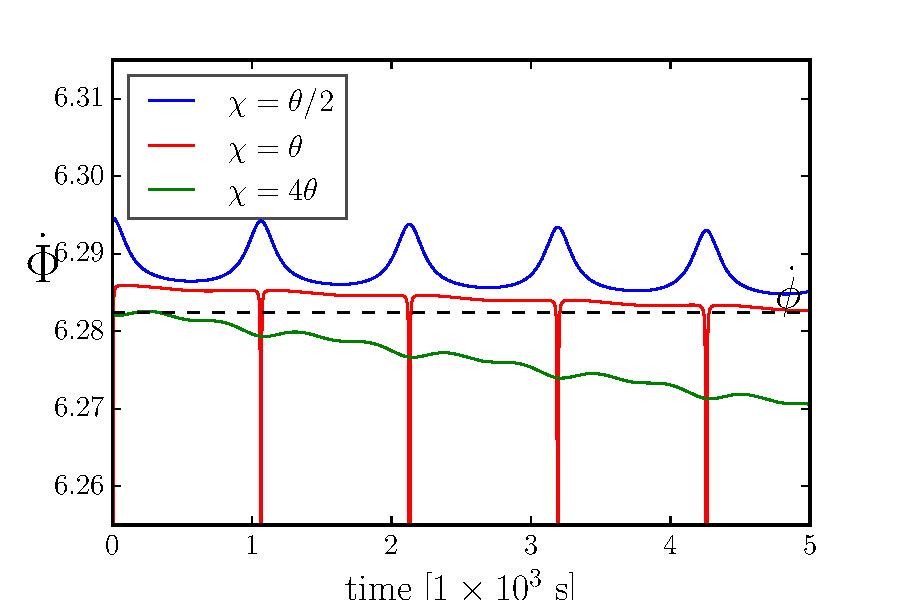
\includegraphics[width=0.7\textwidth]{frequency_variation_with_chi_inc_torque.pdf} \\
%\caption{Variations in the spin-frequency of the dipole $\m$ under torqued precession}
%\label{fig: frequency variations with torque}
%\end{figure}

\section{Physical observables: phase residuals}
\label{sec: timing residuals}

The principle observational quantify reported on for a pulsar is the timing
residual. This is the difference between the measured TOA of a pulse and a
timing model of the pulsar as discussed in Sec.~\ref{sec: pulsar timing
methods}. It is the remaining structure in the timing residual which we
often call `timing-noise' so let us now discuss how this can be calculated
from our numerical model after which we will compare this with analytic
estimates. Note that timing residuals and phase residuals are approximately
equivalent, we will discuss this once we have defined the phase residual.

The azimuthal angle $\Phi$ given in Eqn.~\eqref{eqn: Phi} gives us the phase of
the magnetic dipole. For the observer, the pulsation occurs when the dipole
passes through the plane containing the observer and the angular momentum
vector,  we can always reorient the observer such that the pulsation occurs
every time $\Phi$ is a multiple of $2\pi$. In this way, $\Phi$ is also the
phase of the observed pulsations. To generate $\Phi$ we define the stars
properties i.e. the magnetic field and initial angles, then numerically
evolve equations~\eqref{eqn: ODEs}. The resulting time series of the spin-vector
components and Euler angles are then substituted into Eqn.~\eqref{eqn: Phi} to
generate the exact phase.

Following the methods used by observers, we define our `timing model' as a
a Taylor expansion to the phase about some fixed time $t_{0}$
\begin{equation}
    \Phifit(t; \tref, \phi, \f, \fdot, \fddot) =
    \phi + 2\pi \left(\f(t - \tref) +
                          \frac{\fdot}{2!}(t-\tref)^{2} +
                          \frac{\fddot}{3!}(t-\tref)^{3}
                          \right),
\label{eqn: TR taylor expansion}
\end{equation}
with the timing properties as free parameters.  Note that unlike pulsar
astronomers we do not need to worry about other corrections such as the motion
of the Earth since $\Phi$ is given in the inertial frame.

The phase residual is then the difference between the exact phase
and the fitted phase
\begin{equation}
  \Delta\Phi(t) = \Phi(t) - \Phifit(t; \tref, \phi, \f, \fdot, \fddot).
\end{equation}
We then use a least-squares fitting method to minimise the root mean squared
error of the phase residual. The fitted coefficients $\{\phi, \f, \fdot,
\fddot\}$ constitute out best-fit phase model: the best fit to the data
$\Phi(t)$ of a power law spin-down model.  It is worth noting that a residual
depends on which section of data was used in the fit.

Finally, the phase residual can also be re-scaled to give the timing residual by
calculating the residual as a fraction of a cycle then multiplying by the
period
\begin{equation}
    \Delta T = \frac{\Delta\Phi(t)}{2\pi} P.
    \label{eqn: phase to timing}
\end{equation}
Over a typical observation periods it is possible for the period to
fractionally change due to the spin-down, but the effect is negligible compared
to the other variations considered in this work. Therefore, we will report only
on phase-residuals.

\subsection{Effect of precession on the phase residual}

\citet{Jones2001} analysed the geometric effect that precession will have on
the timing residual. This was done by considering the motion of the magnetic
dipole in the inertial frame as the superposition of motions due to the fast
rotation period and the slow precession. The results must be separated into the
two cases when $\theta > \chi$ and $\theta < \chi$. Of these two the authors
argue that `the wobble angle  of rapidly rotating stars are limited to small
values by the finite crustal breaking strain'. Therefore, the second case
$\theta < \chi$ holds greater physical relevance and so we focus on this region
of parameter space although the numerical code is capable of finding solutions
for either.

\citet{Jones2001} found that, for free precession with $\theta < \chi$,
the phase residual is given by
\begin{equation}
    \Delta\Phi_{49}(t) = -\wobbleangle \cot\chi\cos\left(\dot{\psi}t + \frac{\pi}{2}\right),
    \label{eqn: Jones 49}
\end{equation}
where the subscript here refers to the equation number of \citet{Jones2001}.
For a precessing star $\dot{\psi}$ is given by Eqn.~\eqref{eqn: psi dot} and
the initial value of the cosine argument is $\psi(t=0)=\pi/2$ as derived in
Sec.~\ref{sec: initial conditions}.

Equation \eqref{eqn: Jones 49} is calculated in the absence of any EM torque.
Nevertheless, it is still appropriate when a torque is applied provided
that the geometric effect is stronger that any other (these are discussed in
the next few sections). As such we begin by simulating a NS with the properties
listed in table \ref{tab: PR 49}. Nonphysical values of the
rotation frequency and magnetic field have been used to aid the computational
speed. The resulting phase residual, in cycles, is given in Fig.~\ref{fig:
PR 49}.
\FigureAndTable{49_verification}{PR 49}{
The phase residual in cycles for a simulated NS with the properties described
in the table. This is used to illustrate the
agreement with the magnitude of variations from equation \eqref{eqn: Jones 49}
taken from \citet{Jones2001}.}
This shows strong agreement between the numerical result and the analytic
prediction of Eqn.~\eqref{eqn: Jones 49}. The numerical result does show an
what appears to be a periodic difference with a half period equal to the
data span. This is due to inaccuracies in the fitting procedure and was verified
by changing the data span and observing that the half period shifted accordingly.


\subsection{Effect of precession on the phase residual: electromagnetic amplification}
\label{sec: phase residual torqued}
Considering a vacuum point-dipole spin-down torque \citet{Jones2001} found that
the EM torque can amplify the geometric effect of equation \eqref{eqn: Jones
49}. The magnitude of variation due to EM torque was found to be given by
\begin{equation}
    |\Delta\Phi_{63}| = \frac{1}{\pi}\left(\frac{\tau_{P}}{P}\right)
    \left(\frac{\tau_{P}}{\tau_{S}}\right)
                                    |\Delta\Phi_{49}|
\label{eqn: Jones 63 mag}
\end{equation}
The two ratios of time-scales define an `amplification factor':
\begin{equation}
    \mathcal{A}_{\mathrm{EM}} = \left(\frac{\tau_{P}}{P}\right)
                                \left(\frac{\tau_{P}}{\tau_{S}}\right)
\label{eqn: EM amplification}
\end{equation}
and therefore the phase residuals from the EM torque is given by
\begin{equation}
\Delta\Phi_{63}(t) = \mathcal{A}_{\mathrm{EM}} \Delta\Phi_{49}(t)
\label{eqn: Jones 63}
\end{equation}
The amplification will increases
the magnitude of phase residuals for young pulsars with short periods.

We simulate such a star using the properties in table~\ref{tab: PR 63} noting
that the amplification factor is greater than unity.  The resulting phase
residual is plotted in Fig.~\ref{fig: PR 63} along with the predictions of
Eqn.~\eqref{eqn: Jones 63} and Eqn.~\eqref{eqn: Jones 49}. This clearly demonstrates
that the amplified residuals agree, in magnitude, with the results calculated
numerically. We note that there is some difference in phase between the results,
this is not currently understood.
\FigureAndTable{63_verification}{PR 63}{
The phase residual in cycles for a simulated NS with the properties described
in table \ref{tab: PR 63}. This is used to illustrate the
agreement with the magnitude of variations from equation \eqref{eqn: Jones 63}
taken from \citet{Jones2001}.}

%In figure \ref{fig: TR no torque} we plot the timing residuals as calculated in
%the torque free model for three values of $\chi$. It is worth noting that the
%power law spin down assumes that the star is in fact spinning down; without the
%torque this model can't not spin down. We can however interpret these results
%as the effect of precession on timing residuals in the limit for which the
%variation due to precession is much stronger than the spin down.
%%\begin{figure}[ht]
%%\centering
%%	\includegraphics[width=0.7\textwidth]{Timing_residuals_no_torque.pdf}
%%\caption{Plot of the timing residuals for three angles of $\chi$ in the torque
%%         free model showing different types of behaviour. }
%%\label{fig: TR no torque}
%%\end{figure}
%The results show that the precession induces a periodic variation on the
%precession timescale, the magnitude is proportional to the angle $\chi$. We
%also find the results are dependant on the initial angle $a_{0}$.

%\subsection{Effect of torqued precession on the phase residual: orthogonal rotator}
%
%In analysing observations of free precession \citet{Jones2001} applied the
%model to PSR B1821-11: a pulsar with a strongly periodic residual that has been
%cited as a strong candidate for free precession \citet{Stairs2000}. From the
%variations in pulse shape an estimate can be made of the wobble angle
%$\wobbleangle \sim 3^{\circ}$. Finding that the amplification factor was
%important for this pulsar (it can be calculated to be $\approx 380$),
%\citet{Jones2001} attempted to extract the wobble
%angle by inverting \eqref{eqn: Jones 63}. This yields a wobble angle that
%disagreed with the estimation from a pulse shape variations. The author
%concluded that the strong harmonic periodicity's suggested the dipole was
%nearly orthogonal e.g. $\chi \approx \pi/2$.  This required expansions of the
%phase modulation resulting in an estimate
%\begin{equation}
%    |\Delta\Phi^{75}| = \frac{1}{4\pi} \frac{\tau_{P}^{2}}{\tau_{S} P} \theta^{2}
%    \label{eqn: Jones 75}
%\end{equation}
%
%In figure \ref{fig: PR 75} we simulate the B1828-11 pulsar taking the values
%from \citet{Stairs2000} and modifying them to allow the simulation to complete
%in a reasonable time. The modification was setup such that the amplification
%factor remained the same along with the ratio of timescales. The properties
%of the simulation are given in \ref{tab: PR 75}
%
%\FigureAndTable{75_verification}{PR 75}{
%The phase residual in cycles for a simulated NS with the properties described
%in table \ref{tab: PR 75}. This is used to illustrate the
%agreement with the magnitude of variations from equation \eqref{eqn: Jones 75}
%taken from \citet{Jones2001}.}

\section{Physical observables: spin-down rate}

Like the spin frequency, the spin-down rate observed from a precessing pulsar
will not be only the the secular spin-down of $\omega$, but will also undergo
periodic modulation. Modulations in the spin-down rate for several pulsars have
been observed \citep{Lyne2010, Perera2015} using the method used to do this,
described in Sec.~\ref{sec: pulsar timing methods} involves measured the
spin-down rate in a sliding window.

In our numerical model, the spin-down rate is the second derivative of the
magnetic dipoles azimuthal angle, i.e.  $\ddot{\Phi}$. We can calculate this
directly by differentiating Eqn.~\eqref{eqn: Phi} twice. This will useful in
some analytic circumstances which allow it, and could be done numerically to
calculate the spin-down rate after numerically evolving the original ODEs
of equations~\eqref{eqn: ODEs}.

However, an alternative way to calculate the spin-down rate is to model the
data collection mechanism used by observers: this has the added benefit of
capturing any additional nuances specific to this method. Specifically,
following the method of \citet{Lyne2010}, we fit a second order Taylor
expansions to short sections of data of length $T$ and the resulting
coefficient $\spindown$ is recorded at the mid-point of the section of data.
Repeating this process every $\sim T/4$ in a `sliding-window', we build a
picture of how the spin-down varies with time.  In the following our numerical
results will use this technique which we refer to as the \emph{Lyne-method}.
We choose $T$ such that it is a fraction of the precession period over which we
expect quantities to be modulated. This is consistent with the observers method
where $T$ is chosen in order to resolve the observed modulations.

PSR~B1828-11 is a normal radio pulsar which displays strong periodic modulation
in its spin-down rate. This has been modelled analytically by several authors
\citep{Stairs2000, Jones2001, Link2001, Akgun2006}; in Chapter.~\ref{sec: testing models}
we will discuss the spin-down rate of this pulsar in more detail. \citet{Jones2001}
noted that, as in the case of the timing residuals, the spin-down rate modulations
can be amplified by electromagnetic torques. In the following sections we will
investigate this comparing our numerical model with the analytic models.

\subsection{Effect of torque-free precession on the spin-down rate}
\label{sec: spin-down free precession}

Without an EM torque, the average spin-down rate of the star is zero. However, if
the body undergoes free precession, this will produce periodic modulations about
that average value.
These can be calculated analytically by differentiating Eqn. \eqref{eqn: Phi}
twice. Since the system is torque free the Euler angles evolution's are given
by Eqn.~\eqref{eqn: euler angles torque free evolution} such that
\begin{equation}
    \ddot{\Phi}(t)_{\mathrm{p}} =
%\ddot{\phi}
+ \frac{d}{dt}\left(
        \sin\chi\dot{\psi} \frac{\cos\theta\sin\chi - \sin \psi \sin \theta \cos\chi
}{(\sin\theta \cos \chi - \cos \theta \sin \psi \sin \chi)^{2} + \cos^{2}\psi \sin^{2} \chi}
\right)
\label{eqn: Phi_ddot FP}
\end{equation}
The expanded expression is unwieldy and so we do not report it here.

Additionally, we can easily calculate the  magnitude of variations by
differentiating Eqn.~\eqref{eqn: Jones 49} twice and taking the maximum value
\begin{equation}
    |\Delta\spindown_{\mathrm{p}}| =\frac{\dot{\psi}^{2} \theta \cot\chi}{2\pi}.
    \label{eqn: spin-down variations FP}
\end{equation}

In Fig.~\ref{fig: nu_dot no torque} we plot three curves: the numerical
result obtained using the Lyne-method of calculating the spin-down, the analytic
prediction from Eqn.~\eqref{eqn: Phi_ddot FP}, and the magnitude obtained by
Eqn.~\eqref{eqn: spin-down variations FP}.
\FigureAndTable{nu_dot_no_torque}{nu_dot no torque}{ Modulations in the
    spin-down rate due to free precession. The solid black line is the numerical
    solution, in blue we show the analytic prediction of the magnitude of
    modulations due to free-precession as given by Eqn.~\eqref{eqn:
    spin-down variations FP}, and the red-dashed line indicates the analytic
    prediction of Eqn.~\eqref{eqn: Phi_ddot FP}}
The variations seen in Fig.~\ref{fig: nu_dot no torque} are the result of
free precession. As there is no torque, the average spin-down rate is zero. However,
due to precession the magnetic dipole performs a slow rotation about the
deformation axis. During half the cycle it counter-rotates and in the other
half it corotates with the rapid rotation about the angular momentum vector.
The result is a symmetric modulation of the spin-down rate about zero with magnitude
given by Eqn.~\eqref{eqn: spin-down variations FP}.

\subsection{Effect of torqued precession on the spin-down rate}
In this section we will develop analytic models for the periodic variations due
to precession under an EM torque. This problem has been considered before in
the context of PSR~B1828-11, we will expand on these results and compare the
analytic models with the numeric results calculated using the Lyne-method.

When we include the EM torque, the first effect we observe is that we will have
a non-zero average spin-down rate.  We can calculate this directly from the
power-law braking index model with $n=3$: rearranging Eqn.~\eqref{eqn: surface
magnetic field} for $\dot{\Omega}$ we have
\begin{equation}
    \dot{\Omega} = -\frac{B_{0}^{2}R^{6} \sin^{2}\alpha \Omega^{3}}{6I_{0}c^{3}},
\end{equation}
written in terms of the model parameters this is
\begin{equation}
\dot{\nu} = -\frac{1}{3\pi}\frac{R \Omega^{3}}{c} \sin^{2}\alpha \epsA.
\end{equation}

In the dipole spin-down model the second-order spin-down rate is given
approximately by
\begin{align}
\ddot{\nu} \sim \frac{|\dot{\nu}|}{\tauAge}
\end{align}
As the spin-down age of typical neutron stars is much longer that the time
which we observe pulsars for $\sim 10$~yrs, the secular variation in
$\dot{\nu}$ due to $\ddot{\nu}$ over these observations times are
correspondingly small. Therefore, we can take the initial value of $\dot{\nu}$
as a good estimate for the average spin-down rate
\begin{align}
\langle\dot{\nu}\rangle \approx -\frac{1}{3\pi}\frac{R \Omega_{0}^{3}}{c} \sin^{2}\alpha \epsA
\label{eqn: spin-down initial EM}
\end{align}
In this expression, $\alpha$ is the angle between the spin-vector and the
magnetic dipole. For small wobble angles, the angle $\hat{\theta}$ (see figure
\ref{fig: reference plane}) is vanishingly small and so we can approximate
$\alpha \approx \chi$ such that the average spin-down rate is
\begin{equation}
    \langle \dot{\nu}\rangle = -\frac{1}{3\pi}\frac{R \Omega_{0}^{3}}{c} \sin^{2}\chi \epsA
    \label{eqn: spin-down average}
\end{equation}

This expression will give us the average spin-down under an EM torque. If the
star precesses, then the actual spin-down will be modulated about this values
due to precession as seen in Fig.~\ref{fig: nu_dot no torque}. If the EM torque
is sufficiently weak (we will define this precisely in a moment) then the full
spin-down rate can be modelled by adding the modulations of Eqn.~\eqref{eqn: Phi_ddot FP}
onto Eqn.~\eqref{eqn: spin-down average}. However, we will now demonstrate that when
the torque is strong, just as \citet{Jones2001} found for the timing residuals,
the spin-down rate modulations will be amplified by the torque.

Starting with a vacuum point-dipole spin-down torque \citet{Jones2001}
demonstrated that the magnitude of modulations of the spin-down rate under is
\begin{equation}
    |\Delta\ddot{\Phi}_{58}| \approx -2k\Omega^{3} \theta \sin\chi \cos\chi,
\end{equation}
here the subscript refers to the relevant equation in \citet{Jones2001}. Taking
this expression we can manipulate it as follows
\begin{align}
    |\Delta\ddot{\Phi}|^{58}
    & \approx 2k\Omega^{3} \theta \sin\chi \cos\chi & \\
    & \approx 2 \frac{\ddot{\Phi}}{\sin^{2}\alpha} \theta \sin\chi\cos\chi &
    \mathrm{if }\; \alpha \approx \chi \\
    & \approx 2 \ddot{\Phi}\theta \cot\chi &
    \tauS = \left| \dot{\Phi} / \ddot{\Phi}\right| \\
    & \approx 2 \frac{\dot{\Phi}}{\tauS} \theta \cot\chi &
    P/\tauP = \dot{\psi}/\dot{\Phi} \\
    & \approx 2 \dot{\psi}^{2}\left(\frac{\tauP}{P}\right) \frac{1}{\dot{\psi}} \frac{1}{\tauS} \theta \cot \chi & \dot{\psi} = \frac{2\pi}{\tauP} \\
    & \approx \frac{1}{\pi}\dot{\psi}^{2}\left(\frac{\tauP}{P}\right)\left(\frac{\tauP}{\tauS}\right) \theta \cot\chi
    \label{eqn: spin-down variations FP EM}
\end{align}
Here we have shown that, just like for the timing residuals, the EM torque can
amplify the spin-down modulation by a factor $\mathcal{A}_{\mathrm{EM}}$ as
defined in Eqn.~\eqref{eqn: EM amplification}. In the following two sections
we will investigate how precession effects the spin-down rate with and without
this amplification factor.

\subsubsection{Geometric dominated spin-down modulation}

When $\Aem < 1$, the geometric variations in the
spin-down studied in Sec.~\ref{sec: spin-down free precession} will dominate.
We can derive an ad-hoc analytic expression by allowing
$\ddot{\phi}$ in Eqn.~\eqref{eqn: Phi_ddot FP} to be non-zero and given
exactly by $\ddot{\phi} = 2\pi\langle\dot{\nu}\rangle$, where the average
rate is given in Eqn.~\eqref{eqn: spin-down average}. Combining this with the
geometric modulations, the analytic prediction is given by
\begin{equation}
    \ddot{\Phi}(t) = 2\pi \langle\dot{\nu}\rangle + \frac{d}{dt}\left(
        \sin\chi\dot{\psi} \frac{\cos\theta\sin\chi - \sin \psi \sin \theta \cos\chi
}{(\sin\theta \cos \chi - \cos \theta \sin \psi \sin \chi)^{2} + \cos^{2}\psi \sin^{2} \chi}
\right)
\label{eqn: 1238}
\end{equation}

In Fig.~\ref{fig: nu_dot with torque} we verify that this analytic calculation
agrees with the numerical calculation found by applying the Lyne-method. We
have set the system up such that  $\mathcal{A}_{\mathrm{EM}} = 0.42$. This
shows the non-zero average spin-down due to the EM torque, given by
Eqn.~\eqref{eqn: spin-down average}, and the modulation about this due to the
geometric variations of free precession.

\FigureAndTable{nu_dot_with_torque}{nu_dot with torque}{
Modulation in the spin-down rate due to precession. The solid black line
indicates the numerical solution including a torque; the solid red line indicates
the approximate average spin-down rate due to the EM toque as calculated
from equation \eqref{eqn: spin-down initial EM}; the blue lines indicate
the magnitude of modulation about the average spin-down due to precession; finally
the red-dashed line is the prediction of Eqn.~\eqref{eqn: 1238}.}.

\subsubsection{EM torque amplification of the spin-down modulation}
When $\Aem > 1$, the spin-down modulations amplified by
the torque dominate. We can generate an analytic prediction for this by substituting
Eqn.~\eqref{eqn: Phi_dot} and Eqn.~\eqref{eqn: Theta 2} into the vacuum point-dipole spin-down
torque:
\begin{align*}
\ddot{\Phi} = {} & k \dot{\Phi}\sin^{2}\Theta \\
            = {} & -\frac{2R}{3c} \epsA
                   \left(\dot{\phi}
                         +\frac{\dot{\psi}\sin(\chi)
                                (\cos\theta\sin\chi - \sin \psi \sin \theta \cos\chi)
                               }{
                                (\sin\theta \cos \chi - \cos \theta \sin \psi \sin \chi)^{2}
                         + \cos^{2}\psi \sin^{2} \chi}\right)^{3} \\
            &  \hspace{18mm}  \times  \sin^{2}\left(\cos^{-1}\left(
                     \sin\theta\sin\psi\sin\chi + \cos\theta\cos\chi\right)\right)\\
    = {} & -\frac{2R}{3c} \epsA
    \left(\dot{\phi}+\frac{\dot{\psi} \sin(\chi)(\cos\theta\sin\chi
          -\sin \psi \sin \theta \cos\chi)}
         {(\sin\theta \cos \chi - \cos \theta \sin \psi \sin \chi)^{2}
         + \cos^{2}\psi \sin^{2} \chi}\right)^{3} \\
   & \hspace{18mm} \times \left(\sin\theta\sin\psi\sin\chi + \cos\theta\cos\chi\right)
\end{align*}
where we are implicitly assuming $\theta=\mathrm{const.}$, this is not true
when we include the EM torque. However, provided the variations are small we
can assume it as a first approximation.  Finally, we also assume that the other
Euler angles are approximately the same as in the torque free case, that is:
 \begin{align}
\begin{split}
     \ddot{\Phi} =&-\frac{2R}{3c} \omega_{0}^{3}\epsA
     \left(1 -  \epsI\frac{ \sin(\chi)(\cos\theta\sin\chi - \sin \psi \sin \theta \cos\chi)
     }{(\sin\theta \cos \chi - \cos \theta \sin \psi \sin \chi)^{2} + \cos^{2}\psi \sin^{2} \chi}\right)^{3}\\
     &\hspace{22mm}\times\left(\sin\theta\sin\psi\sin\chi + \cos\theta\cos\chi\right)
     \label{eqn: Phi_dot EM}
\end{split}
\end{align}
In Fig.~\ref{fig: nu_dot with torque EM} we plot the results of a simulation
for which this amplification factor is greater than unity. This demonstrates
that the numerical solution, obtained using the Lyne-method, has variations in
spin-down rate in good agreement with Eqn.~\ref{eqn: spin-down variations FP
EM}.  Furthermore we also show the magnitude of variations about the average
which is predicted by free precession alone, as given in Eqn.~\eqref{eqn:
spin-down variations FP}: this shows that the numerical simulation has larger
variations due to the amplification.
\FigureAndTable{nu_dot_with_torque_EM_amplification}{nu_dot with torque EM}{
EM amplification of the modulation in the spin-down rate due to precession.
The solid black line indicates the numerical solution including a torque; the
solid red line indicates the approximate average spin-down rate due to the EM
toque as calculated from equation \eqref{eqn: spin-down average}; the
blue region indicates the modulation about the average spin-down due to
precession from Eqn.~\eqref{eqn: spin-down variations FP} while the green
region indicates the modulation about as calculated from
Eqn.~\eqref{eqn: spin-down variations FP EM}.}


In this section we have derived some ad-hoc formulae and demonstrated their
agreement with spin-down rate calculated numerically using the Lyne-method. We
do not intend that these ad-hoc formulae are complete and have not quantified
the size of errors due to some of the assumptions made, such as using the
torque-free Euler angle solutions when we in fact did have a torque. Instead,
we simply use them to understand the features of the spin-down rate under the
torque. A complete derivation of the spin-down rate under strong amplification
is given in Sec.~\ref{sec: derivation of the spin-down rate}.

\section{Physical observables: the shape of pulsation}

So far we have considered physical observables which are calculable from the
timing properties of the star: the rate at which pulses occur. However, pulsar
astronomers also discuss the shape of the pulsation by averaging over many
pulses to form an integrated pulse profile. This pulse profile is sensitive to
both the geometry of the beam itself, and the angle made between the beam and
the observer.  In this section we will discuss the variations in this angle due
to precession and then discuss the variations in the observed pulse assuming a
beam geometry.

\meta{Link to earlier section}

Let us define an observer fixed in the inertial frame such that they
maintain a constant angle $\iota$ with the angular momentum of the star $\J$.
For this observer, a pulse can be defined as the moment the dipole cuts through
the plane containing them and the angular momentum vector. At this moment, the
angle between them and the dipole will be determined by both $\iota \in [0, \pi]$ and
$\Theta \in [0, \pi]$. In particular, the angle between the observer and the beam
is given by
\begin{equation}
\Delta\Theta = \Theta - \iota
\label{eqn: delta Theta}
\end{equation}

Since $\iota$ is fixed, variations in $\Delta\iota$ come solely from variations
in the polar angle $\Theta$. 

\subsection{Variations in the pulse intensity}
The intensity of radiation received by an observer will depend on the
orientation of the magnetic dipole with respect to the observer and the beam
geometry. It will be maximal when pointing directly at the observer and
presumably fall off as the angle between the two grows. For each rotation of
the star, the intensity will peak when the beam cuts the plane containing the
observer and the angular momentum vector, in this instance the angle between
the two is given by Eqn.~\eqref{eqn: delta Theta}. If the star is precessing
then the periodic pulses of intensity due to the azimuthal rotation of the star
will be modulated by the slower variations in $\Theta$ seen in Fig.~\ref{fig:
polar angle variations}.

To model this we take an observers position as $\Phi_{O}, \iota$ and then
assume the beam geometry follows Gaussian profile with a single conal emission.
This could later be adapted to include a coral emission.  For such a model of
the beam geometry, the intensity of pulsations will vary with the angular
separation of the vector from the centre of the star to the observer and the
magnetic dipole vector. By considering the intersection of these vectors with
the unit sphere, the angular separation can be shown to be
\begin{equation}
\Delta\sigma = \cos^{-1}\left(\sin(\Theta)\sin(\iota) +
                             \cos(\Theta)\cos(\iota)\cos(\Phi - \PhiO)\right)
\label{eqn: angular sep inv cos}
\end{equation}
Then, taking a Gaussian beam geometry, the intensity of the pulse will be given by
\begin{equation}
A(\Theta, \Phi, \iota, \PhiO, \sigmaB) =
A_{0} \exp\left(-\frac{\Delta\sigma^{2}(\Theta, \Phi, \iota, \PhiO)}{2\sigmaB^{2}}\right)
\label{eqn: gaussian beam intensity}
\end{equation}
where $A_{0}$ is some constant amplitude, $\sigmaB$ is a measure of the
angular beam width.

Given a value for $A_0$ and $\sigmaB$, we can use a numerical solution to the
governing ODEs to simulate this pulse intensity exactly This is done in
Fig.~\ref{fig: intensity variation} for a system where the variations in
$\Theta$ occur on a time scale not much longer than the pulse period. This
nonphysical simulation is intended to show the modulation of the individual
pulsations due to precession.
\begin{figure}[htb]
\centering
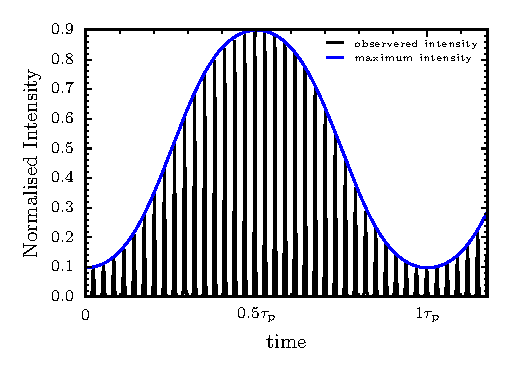
\includegraphics[width=.7\textwidth]{intensity_variation}
\caption{Amplitude variation using a 2D Gaussian emission.}
\label{fig: intensity variation}
\end{figure}
We can also predict the maximum pulse intensity at any given instance by setting
$\Phi=\PhiO$, then simplifying we find that
\begin{align}
A_{\mathrm{max}}(\Theta, \Phi, \iota, \sigmaB) =
A_{0}\exp\left(\frac{-(\Theta-\iota)^{2}}{2\sigmaB^{2}}\right),
\label{eqn: A max}
\end{align}
this is also shown in Fig.~\ref{fig: intensity variation}.

\subsection{Variations in the beam-width}
It is unlikely that the variations seen in Fig.~\ref{fig: intensity variation}
will ever be visible, over longer time-scales of course, in nature. This is because
in real observations the intensity will also be subject to variations in the
amount of dispersion from the interstellar medium. Therefore, pulsar astronomers
do not typically report on intensities themselves, but characterise the pulsation
by their beam-width. This is the width of the pulse at some percentage $p$ of
the observed maximum intensity. Note that this is not the maximum intensity that
the beam produces, $A_0$, but the maximum at that instant in time which is
given by Eqn.~\eqref{eqn: A max}

To model the beam-width we first note that in Eqn.~\eqref{eqn: gaussian beam intensity},
$\Theta$ varies on the slow precession timescale, while $\Phi$ varies on the
rapid spin timescale: we are looking to measure the variations with respect to
the slow precession timescale.  The pulse width is measured by the time spent
above a percentage $p$ of the maximum pulse amplitude, this can be defined as
\begin{align}
A(\Phi, \Theta, \ThetaO, \PhiO, \sigmaB) > A_{\textrm{max}} \frac{p}{100}.
\end{align}
Substituting in Eqn.~\eqref{eqn: gaussian beam intensity} and Eqn.~\eqref{eqn: A max}
then rearranging yields
\begin{equation}
\cos(\Phi - \PhiO) < \frac{
\cos\left(
\sqrt{-2\sigmaB^{2} \ln\left[\frac{p}{100}\frac{A_\textrm{max}}{A_0}\right]}\right) - \sin(\Theta)\sin(\Theta)}
                          {\cos(\Theta)\cos(\ThetaO)}
\label{eqn: 6737}
\end{equation}
where we note that $A_\textrm{max}$ is not a constant, but will evolve with the
polar angle $\Theta$.

Lets consider a single rotation with the magnetic dipole starting and ending in
the antipodal point to the observers position. During this rotation, $\Phi -
\PhiO$ increase between $-\pi$ and $\pi$, and so the left hand side of the
inequality is a simple cosine function as illustrated in Fig.~\ref{fig:
CosineIllustration}.  Since we expect $\Theta$ to vary slowly compared to the
rotation period we can, over a single pulsation, think of $\Theta$ as a
constant; then the whole right hand side of inequality~\eqref{eqn: 6737} is a
constant. In Fig.~\ref{fig: CosineIllustration} we illustrate this constant
along with the evolution of the left hand side: the fraction of the rotation
for which the cosine is less than the constant, i.e. inequality~\eqref{eqn: 6737}
is satisfied, defines the beam-width.
\begin{figure}[ht]
\centering
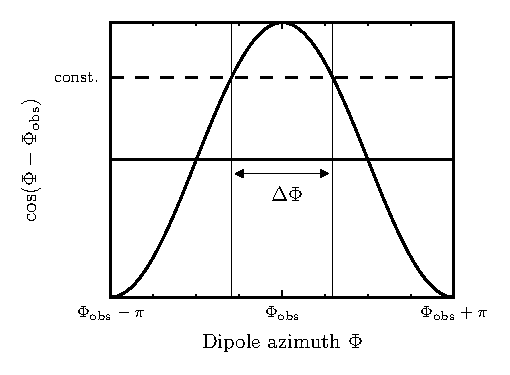
\includegraphics[width=.5\textwidth]{CosineIllustration.pdf}
\caption{Illustration of the inequality in equation \eqref{eqn: 6737} the constant
         value represents the right hand side of this equation. The
         width $\Delta\Phi$ indicates the angular period during which inequality
         is satisfied.}
\label{fig: CosineIllustration}
\end{figure}

We can calculate the beam width by first calculating the angular width $\Delta\Phi$
when the inequality is not satisfied:
\begin{equation}
    \Delta\Phi = 2\cos^{-1}\left(
                \frac{\cos\left(\sqrt{2\sigmaB^{2} \ln(f)}\right) - \sin(\Theta)\sin(\Theta)}
                          {\cos(\Theta)\cos(\ThetaO)}
                      \right).
\end{equation}
Then the angular fraction at which the inequality \emph{is} satisfied is given by
$2\pi - \Delta\Phi$. To convert this into the beam-width reported by pulsar
astronomers we multiply by the pulse period
\begin{align}
    W_{p} & = P \frac{2\pi - \Delta\Phi}{2\pi}\\
          & = \frac{1}{\pi \dot{\Phi}}\left(1 -
               \cos^{-1}\left(
                   \frac{\cos\left(\sqrt{2\sigmaB^{2} \ln(\frac{100}{p})}\right) - \sin(\Theta)\sin(\Theta)}
                          {\cos(\Theta)\cos(\ThetaO)}
                      \right)
                  \right)
\label{eqn: Wp}
\end{align}
where $P$ is the spin period which we have then written in terms of the spin
frequency and $p$ is the percentage of beam width.

To demonstrate what a beam-width can look like in Fig.~\ref{fig: Pulse width
modulation} we plot the beam-width calculated from a numerical simulation and
Eqn.~\eqref{eqn: Wp}. Additionally, we show the variation of $\Theta$ for the
simulation and mark on $\iota$, the polar angle of the observer in the inertial
frame.
\begin{figure}[ht]
\centering
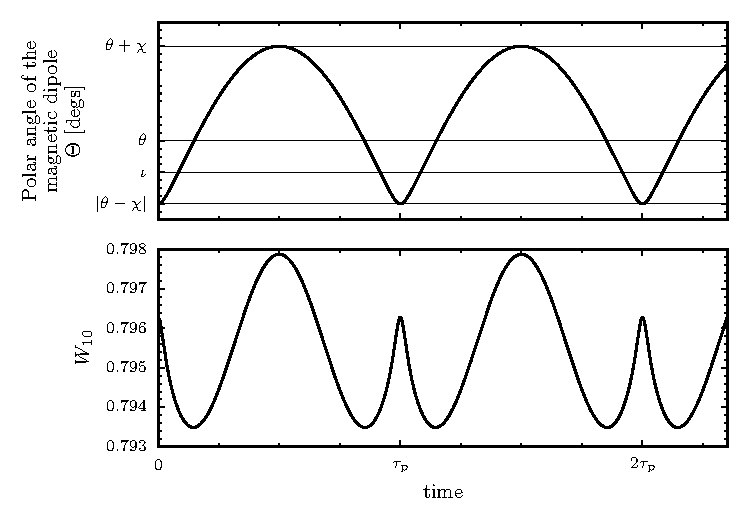
\includegraphics[]{Pulse_width_modulation.pdf}
\caption{Simulation results for the polar angle $\Theta$ and $W_{10}$, a
measure of the observed beam-width as calculated from Eqn.~\eqref{eqn: Wp}.}
\label{fig: Pulse width modulation}
\end{figure}
This shows that there is periodic modulation of the beam-width, with an
interesting two-peak structure. This structure can be understood by realising
that the polar angle of the dipole $\Theta$ `passes over' the observer such
that for some of the precessional phase the observer sees the beam from below,
and other from above. This leads to the two-peaked structure due to the
symmetry of the emission geometry.


\section{Application: switching and precession}

Recently, some workers in the field \citep{Lyne2010, Perera2015} are suggesting
that quasi-periodic structure observed in pulsar timing residuals is a result
of magnetospheric torque-switching events as described in Sec.~\ref{sec: two
state switching}. In such models, the spin-down periodically switches between
two distinct values and these changes correlate with changes in the beam-width.
These models however are lacking a key feature: the clock which provides the
periodicity. It has been suggested \citep{Jones2012} that it may in fact be
precession which provides this clock. Ultimately, the numerical model developed
in this section could study this effect, for example by implementing a hybrid
model in which propensity for a magnetospheric switch to occur is related to
the angle $\Theta$. In this way, the observed switching would undergo
stochastic resonance as suggested by \citet{Cordes2013} and discussed in Appendix~\ref{app:
stochastic}.

In this section we will present preliminary results on a simplified hybrid model
in which we consider single switching events. We will not connect the switching
to precession, but simply consider a single switch in the torque at some time
$t_{\mathrm{switch}}$; for the time being we set this to be half the
observation period, such that $t_{\mathrm{switch}} = \To/2$.

In the EM dipole spin-down model, the torque has two distinct components: the
regular spin-down component and the anomalous component. This latter term
does not contribute to the spin-down, but as discussed in Sec.~\ref{sec: effective
body frame} will modify the axis of precession. Magnetospheric switching models
are based on evidence that the spin-down rate is switching, therefore the torque
switching must occur in the spin-down component. However, it is unclear if it would
also occur in the anomalous component, to answer this would need a detail model
of each how the magnetosphere reconfigures during a switching. We will not do
this here, but instead investigate a simple phenomenological switching in which we
modify Eqn.~\eqref{eqn: torque} as follows
\newcommand{\Ss}{S_{\mathrm{S}}}
\newcommand{\Sa}{S_{\mathrm{A}}}

\begin{equation}
\mathbf{T} = (1 - \Ss H(t-t_{\mathrm{switch}})) \mathbf{T}_{\mathrm{S}}+
                 (1 - \Sa H(t-t_{\mathrm{switch}})) \mathbf{T}_{\mathrm{A}}
\label{eqn: single switch torque}
\end{equation}
where the subscripts label the spin-down and anomalous components, $S$ is the
strength of switching, and $H(t)$ is the Heaviside step function. In this model
we can control which components are switched by choosing $\Ss$ and $\Sa$
appropriately.

In our model the strength of the EM torque is parameterised
by $\epsA$, related to the surface magnetic field strength by
\begin{align}
    \epsA = \frac{R^{5}}{4I_{0} c^{2}} B_{0}^{2}.
\end{align}
Rearranging Eqn.~\eqref{eqn: surface magnetic field} we can then write the
spin-down rate as
\begin{align}
    \dot{\omega}_{0} & = -\frac{B_{0}^{2}R^{6} \sin^{2}(\alpha) \omega_{0}^{3}}{6 I_{0} c^{3}} \\
    & = - \frac{2 R \epsA \sin^{2}(\alpha) \omega_{0}^{3}}{3 c},
\end{align}
where $\alpha$ is the angle between the spin-vector and magnetic dipole. Since
we expect these to be misaligned in order to observe pulsations, we can take
$\sin^{2}\alpha \approx 1$, then our spin-down rate is approximately
\begin{equation}
    \dot{\nu} = - \frac{R\omega_{0}^{3}}{3\pi c}\epsA.
    \label{eqn: spin-down of epsA}
\end{equation}

From this we can equate the switching in the spin-down rate $\Ss$ directly to
that measured from pulsar observations. That is, from Eqn.~\eqref{eqn: single switch torque}
we have that
\begin{equation}
    \epsA \rightarrow \epsA' = (1-\Ss)\epsA.
\label{eqn: epsA switch}
\end{equation}
during a switching, then the spin-down rate also changes as
\begin{equation}
    \dot{\nu} \rightarrow \dot{\nu}' = (1-\Ss)\dot{\nu}.
\label{eqn: nudot switch}
\end{equation}
during a switching event.


\subsubsection{Minimal precession initial state}
In the following section we will investigate the effects of a single switch, but
we first need to define a `minimal precession' initial state to which the
switch is applied so that we understand the behaviour without the switch.

Precession will not occur when the spin vector is aligned with the axis about
which it rotates. The angle between these two we have defined as the wobble
angle.  For minimal precession we should therefore set this wobble angle to
zero. In all simulations, we consider a biaxial body with the full torque given
by \eqref{eqn: single switch torque}. From our previous discussion on the
wobble angle we can minimise the precession initially by setting the initial polar angle
of the spin vector in the rotating frame to lie along the effective body-frame
axis. In the presence of the anomalous torque this is done with
\begin{equation}
a_{0} = \beta(\epsI, \epsA, \chi),
\end{equation}

In Fig.~\ref{fig: no switching} we illustrate the behaviour of our simulation
in the absence of a switching event; the simulation parameters are listed in
table \ref{tab: NoSwitching properties}, note that the initial polar angle is
exactly the angle $\beta$ which can be calculated using equation \eqref{eqn:
beta}.
\begin{figure}[htb]
\begin{floatrow}
\ffigbox{%
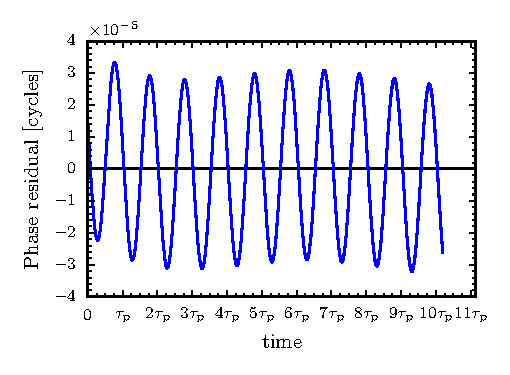
\includegraphics[width=0.5\textwidth]{NoSwitching.pdf}
}{%
    \caption{The phase residual for a minimal precession simulation with no
             switching event.}
  \label{fig: no switching}
}
\capbtabbox{%
  \begin{tabular}{ccl}
\multicolumn{3}{c}{Simulation parameters} \\
\hline
$\omega_0$  &=& 100 rad/s\\
$B_0$  &=& $10^{15}$ G \\
$\chi$  &=& 50$^{\circ}$ \\
$a_0$ &=& -0.78$^{\circ}$ \\
$\mathcal{A}_{\mathrm{EM}}$ &= & $23$
\end{tabular}

}{%
  \caption{}%
  \label{tab: NoSwitching properties}
}
\end{floatrow}
\end{figure}
Notably this minimal precession solution does show some precession with phase
residuals $\sim 10^{-4}$. This is because the spin-down torque produces a wobble
in the angular momentum vector and as a result the wobble angle is not truly
zero. In addition to this precessional wobble, there is also an inaccuracies
in the polynomial fitting which produces structure with a period equal to that
of the observation span.

We will now setup simulations of this `minimal precession` NS, and then
manually switch the torque. We choose a NS where the EM torque amplification
is important.

\subsection{Switching in the spin-down torque only}
We now consider manually switching the spin-down torque halfway though the
simulation, with no switch occurring in the anomalous component.
That is we set
\begin{align}
    t_{\mathrm{switch}} = \frac{\To}{2}, &&& \Ss = 0.4, &&& \Sa = 0.0,
\end{align}
such that halfway though the simulation the spin-down torque is reduced by a
fraction $0.4$ while the anomalous torque remains unaffected.

In Fig.~\ref{fig: switching without anom} we plot the phase residuals from
this simulation. In the top plot is the residual as calculated over the entire
observation period. We find a single periodic variation which is a direct result
of the sudden change in the spin-down rate. The precession features which existed
in the initial minimal precession are swamped by the larger variations due to
the switch. To study this simulation further,
in the lower plot we plot two residuals: the first is calculated
in the region $[0, t_{\mathrm{switch}}]$ and the second in $[t_{\mathrm{switch}}, \To]$,
the are marked by different colours.
Because the switch does not occur in either of these periods we can resolve the
free precession during each period and note that the precession modulation is
in fact smaller after the switch.
\begin{figure}[htb]
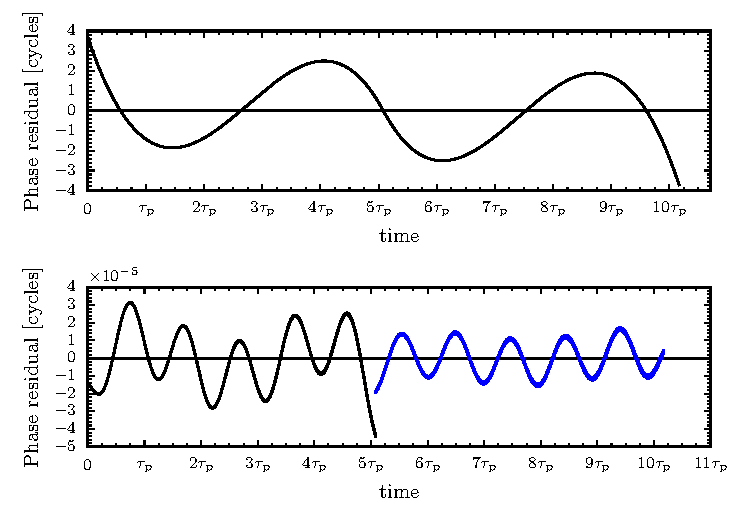
\includegraphics[width=.5\textwidth]{SwitchingWithoutAnomTorque}
\caption{Phase residuals for a simulation with a single switch in the spin-down
torque. In the top plot we show the residual calculated using the whole observation
time, in the bottom plot is the separate residuals calculated in the region before
and after the switch.}
\label{fig: switching without anom}
\end{figure}
This reduction in the size of modulations is because the precession is due to
the spin-down torque wobbling the angular moment vector. After the switch the
spin-down torque is reduced by a factor $\Ss$ and therefore the size of the
modulation is similarly reduced.

\subsection{Switching with the anomalous torque}
We now consider manually switching both the spin-down and anomalous torque
halfway though the simulation.  That is we set
\begin{align}
    t_{\mathrm{switch}} = \frac{\To}{2}, &&& \Ss = \Sa = 0.01
\end{align}

In a similar fashion to Fig.~\ref{fig: switching without anom} we show first
the total residual in the top plot of Fig.~\ref{fig: switching with anom}, and
then the individual residuals in the lower plot. Again the overall phase residual
shows strong periodic modulation resulting from the switch. In contrast to the
spin-down only switching, the amount of precession when considered before and
after the glitch now increases.

To understand this, recall that we begin with a minimal precession state, where
$\theta = \beta$ and the precession results from effect of the spin-down
torque.  After the switch, we have changed the size of the anomalous torque and
hence we have modified the effective rotating frame and the angle $\beta$. This
means that after the switch the wobble angle is no longer in a minimal
precession configuration.
This generates a significantly larger wobble angle producing a significant
increase in the phase residuals fitted in the post-switch period. The effect is
not observable when fitting to the entire simulation period since the switching
event remains dominant. In the next section we will calculate this new wobble
angle.

\begin{figure}[htb]
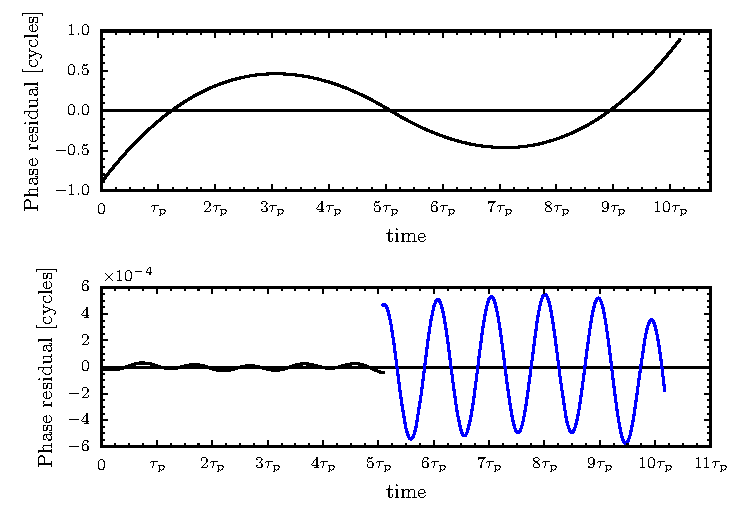
\includegraphics[width=.5\textwidth]{SwitchingWithAnomTorque} \caption{Phase
residuals for a simulation with a single switch in the spin-down and anomalous
torque. In the top plot we show the residual calculated using the whole
observation time, in the bottom plot is the separate residuals calculated in
the region before and after the switch.}
\label{fig: switching with anom}
\end{figure}

\subsubsection{Calculating the new wobble angle after a switch}
We now calculate the change in wobble angle and hence phase-residual variations
after switching a fraction of the anomalous torque.

The two-state switching changes the value of $\epsA$ according to
Eqn.~\eqref{eqn: epsA switch}, which in turn redefined the effective rotating frame
as defined in Sec.~\ref{sec: effective body frame}. A non-precessing NS at an
angle $\beta(\epsI, \epsA, \chi)$ will, after an anomalous torque switch by a fractional
amount $\Sa$, no longer be aligned with the rotating frame axis. This is
because the effective rotating frame will have shifted to $\beta' = \beta(\epsI,
\Sa\epsA, \chi)$. As a result, we should expect the previously
non-precessing NS to begin precessing after a torque switching event.

The NS will precess at the usual precession frequency in a cone  of half-angle
\begin{equation}
    \Delta\beta(\epsI, \epsA, \chi, \Sa)=|\beta - \beta'|,
\end{equation}
about the new effective body-frame axis.  The expression for $\Delta \beta$ is
not easily amenable to analytic calculation, but can easily be explored
graphically.  This is done in Fig.~\ref{fig: DeltaBetaPlot} for several choices
of $\Sa$. This illustrates that the new precession angle after a switch can be
as much as a few degrees although it tends to zero in the limit $\epsI \gg
\epsA$.
\begin{figure}[htb]
    \centering
    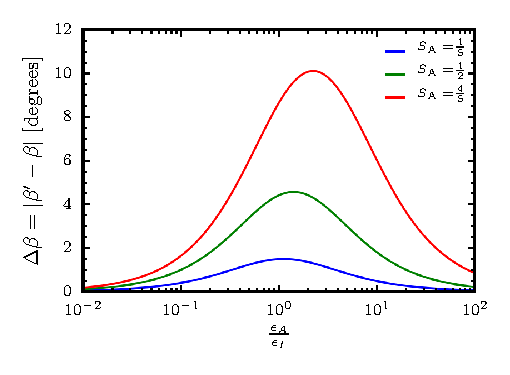
\includegraphics[]{DeltaBetaPlot}
    \caption{Illustrating the magnitude of the precession angle after switching
        due to the new rotation of the effective rotating frame. We plot the half-angle
        ($\Delta\beta$) of the precession cone as a function of the ratio
    $\epsA/\epsI$. Typically we expect real stars to have $\epsA < \epsI$.}
    \label{fig: DeltaBetaPlot}
\end{figure}

A simple application of this work is to apply our findings to PSR~B1828-11,
which was interpreted by \citet{Lyne2010} as undergoing switching with a fractional
change in the spin-down rate given by
\begin{align}
\frac{\Delta\dot{\nu}}{\dot{\nu}} = 0.0071
\end{align}
Manipulating Eqn.~\eqref{eqn: nudot switch}, we see that that
\begin{align}
|\Ss| = \frac{\Delta\dot{\nu}}{\dot{\nu}}
\end{align}
Using data from the ATNF catalogue \citep{ATNF}, B1828-11 has a frequency
$\nu = 2.47$~Hz, a spin-down rate $\dot{\nu}=-3.65\times10^{-13}$~Hz/s.
Rearranging Eqn.~\ref{eqn: spin-down of epsA} we then have
\begin{align}
\epsA^{B1828-11} = \frac{c}{8\pi R\nu^{3}}\dot{\nu} \approx 2.89 \times 10^{-11}
\end{align}

Now in this interpretation, $\epsI$ is unconstrained for B1828-11 since the
periodic modulations are assumed to be resulting from switching and not
precession. Nevertheless, we numerically maximise over $\epsI$ to find
\begin{align}
\Delta\beta_{\textrm{max}}(\epsI=2.89\times10^{-11}, \epsI=2.87\times10^{-11})
= 0.048 \textrm{ degs}
\end{align}
This is the new wobble angle which must occur every time B1828-11 undergoes a
switching event, if the switch also occurs in the anomalous torque. This
therefore provides a method to probe how the switching mechanism works by
looking at timing residuals in the post-switch timing data to check for
any signs of precession.

\section{Conclusions}

In this chapter we have developed a method to simulate observable properties of
neutron stars by evolving the governing system of ODEs. These equations
\eqref{eqn: ODEs} contain both the components of the spin vector in the
rotating frame and the Euler rotation angles required to transform from
the rotating frame to the inertial frame. This step is important since it is in
this reference frame that observers see the peculiar features of precession.

We developed an intuitive model for how the magnetic dipole, along which EM
radiation is emitted, moves in the inertial frame. Comparing with analytic
models where possible, we showed how the calculate from the motion of the
dipole the evolution of the stars timing properties (the phase, frequency, and
spin-down rate) and how to calculate features of the beam shape such as the
beam-width.

Finally, we used the phase residuals to investigate the effect of a simple torque
switching model in which the components of the torque instantaneously change.
This was done to model, in a simple way, the magnetospheric switching which is
proposed by \citet{Lyne2010} as an explanation of the periodic modulation of
B1828-11. Our numerical model is ideally suited to this task as it captures the
complicated feedback between precession and the changing torque.
A future application of this model is to link the switching to the precessional
phase in a probabilistic way as proposed by \citet{Jones2012}. In this way
precession provides the clock to the switching. We feel that, by virtue of
being probabilistic, such a system will display stochastic resonance as first
described by \citet{Cordes2013}.

\biblio

\end{document}
